\renewcommand{\thefigure}{\Asbuk{section}.\arabic{figure}}
\renewcommand{\thetable}{\Asbuk{section}.\arabic{table}}
\renewcommand{\thelstlisting}{\Asbuk{section}.\arabic{lstlisting}}

\begin{landscape}
\section*{ПРИЛОЖЕНИЕ A \\ (справочное) \\ <название приложения>}

\setcounter{section}{1}
\setcounter{figure}{0}
\setcounter{table}{0}
\setcounter{lstlisting}{0}

В редких случаях бывает удобно выделять объемные рисунки и таблицы, а также листиниги в приложения:
  
\begin{figure}[h]
\centering
  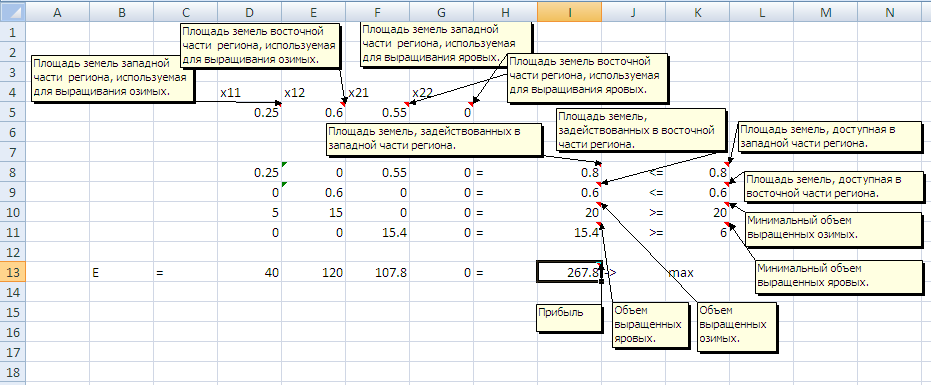
\includegraphics[width=1\linewidth]{pic/excel}
  \caption{Рабочий лист Excel с результатами решения базовой задачи линейного программирования}
\end{figure}

\end{landscape}

\newpage
